\section{Method}
Both the spectrums and the images will be analysed using spectrometer methods, this will open up for the opportunity to pre-process spectral and spatial data in the same way. We will then hopefully be able to compare the data more directly. The spectrometer processing method we want to use is relative reflectance ($RR$). Since this method is also being used with the spectrometer, it will be denoted $RR'$ whenever it is used for imaging. As can be seen from (\ref{eq:relative_reflectance}), relative reflectance is done by dividing the interesting values with a reference. The translation to image processing must be to divide every image pixel with a pixel value from a reference image. For comparing values with the spectrometer it is fully ok to do this division as long as the reference image is non-zero for all pixels. For that reason it is important with a well lit and preferably white background. 


One problem with this method is that images can only be visualized as a set of pixels, each pixel consisting of three integers between 0 and 255, i.e. the colors blue, green and red. Therefore we divide the division into to two cases when visualizing; reference divided by image and image divided by reference. The product will be denoted $RR'_{negative}$ for the reference divided by image case, and $RR'_{positive}$ for the image divided by reference case. The processing can be view in figure \ref{fig:image_visualization_program_flow}. Here $A$ is the image with an object and $A_0$ is the reference image. To deal with noise in the system, a noise limit is put in place before doing the division. This noise limit ensures that the difference between the image to be analysed and the reference is large enough to be assumed as a signal and not noise. This paper will later find the noise limit value with the infamous trial and error method. 

\begin{figure}[h]
    \centering
    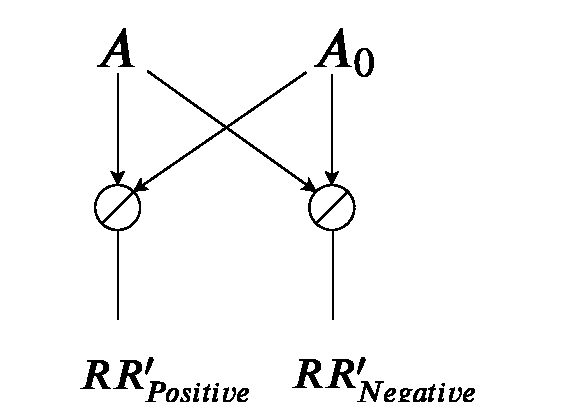
\includegraphics[width=0.5\textwidth]{figures/image_program_flow.pdf}
    \caption{Image visualization process flow}
    \label{fig:image_visualization_program_flow}
\end{figure}


\subsection{Spectrum processing}
\label{sec:spectrum_processing}

\begin{figure}[h]
    \centering
    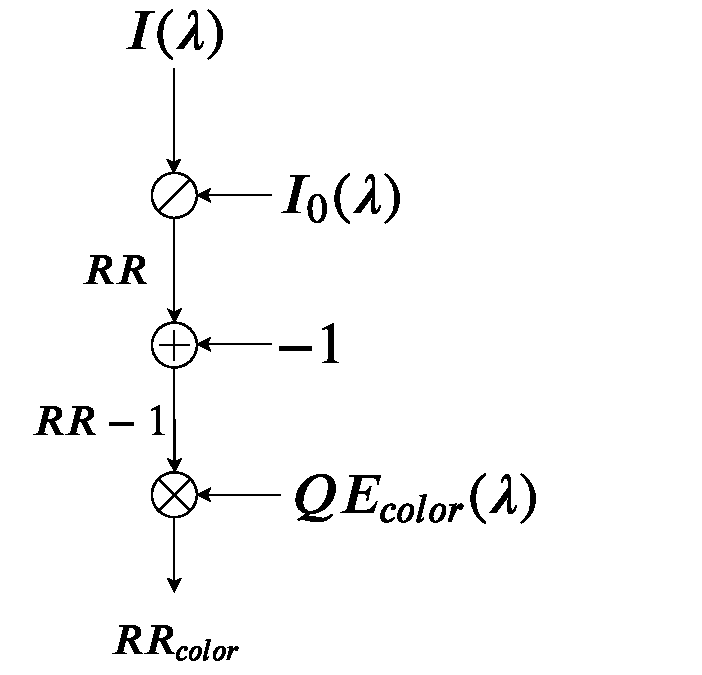
\includegraphics[width=0.5\textwidth]{figures/thesis_program_flow.pdf}
    \caption{Spectrum process flow}
    \label{fig:spectrum_process_flow}
\end{figure}

\subsection{Correlating Spectrometer to Camera}
\label{sec:method_correlating_spectrum_to_camera}
To get an idea of how well calibrated the camera is to the spectrometer and vice versa I propose the following calculation: 
Take the spatial average across the image from the camera and compare it with the spectral average of the spectrometer. This comparison should be done by plotting the spectral average values of the spectrums on the y-axis, and the spatial average values on the x-axis. This allows for any correlation to be easily spotted. 

The process of comparing is shown in figure \ref{fig:correlating_spectrum_and_image}. The $\oslash$ symbol denotes the Hadamard division that was introduced in section \ref{sec:hadamard_division}, and the $\otimes$ symbol was introduced in \ref{sec:hadamard_product}. 

\begin{figure}[h]
    \centering
    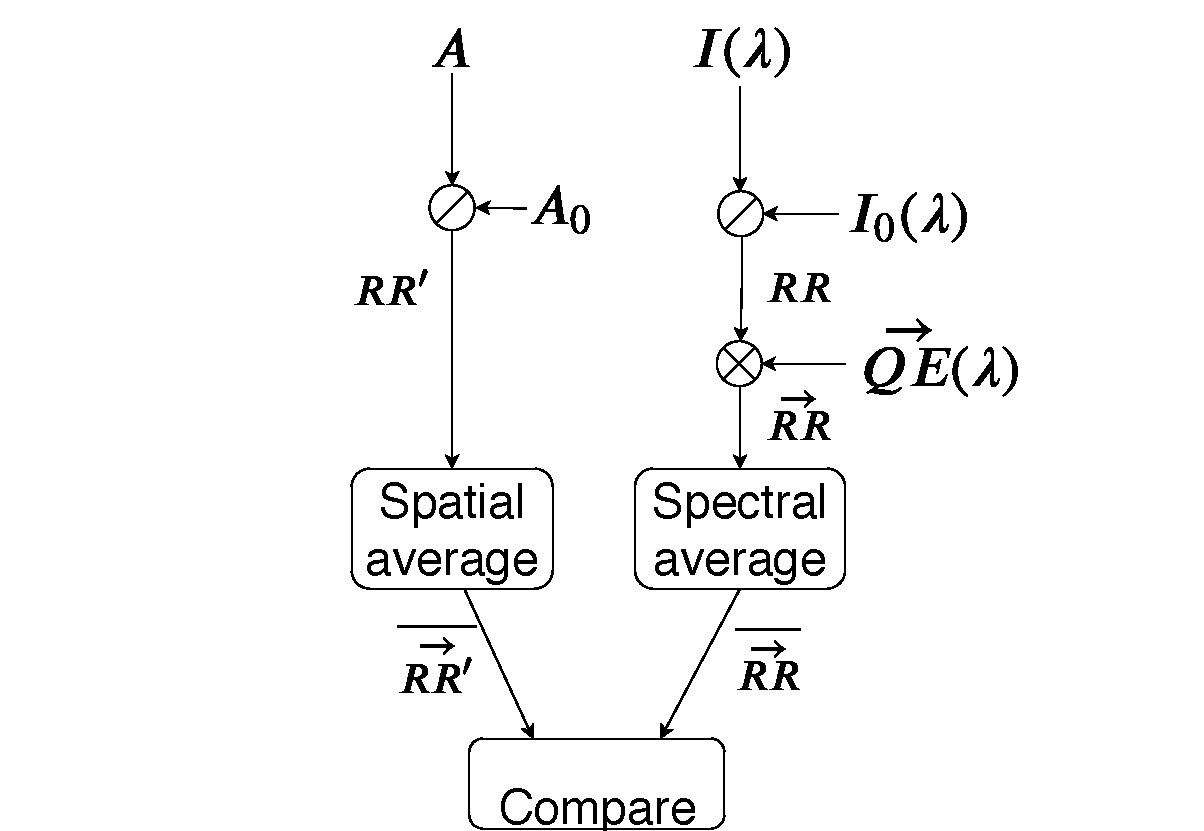
\includegraphics[width=0.75\textwidth]{figures/image_comparison_with_spectrometer.pdf}
    \caption{Correlating value between image and spectrum}
    \label{fig:correlating_spectrum_and_image}
\end{figure}


\subsection{Light illumination}
Light is a crucial part of this project, as it is the source of input for both the camera and the spectrometer. It's also the link between the two sensors. The choosing of a light source that can support both sensor types is therefore paramount. The camera is less selective on the spectral properties of the light source as it only requires a light source that is approximately white, i.e. have similar amounts of red, green and blue "wavelengths". It is however more selective in the spatial region as it can arise more problems for the camera if the lighting creates a lot of shadows or local problems like strong specular reflection making the pixel go into saturation. As implied the spectral properties of the light is more important for the spectrometer. For the spectrometer we want the spectrum to be as flat as possible. 

%TODO: The characterization of the light source will be based on considerations from \cite{martinPracticalGuideMachine}, but also unfortunately be limited by available sources at the lab.
 % This paper provides a longer checklist, that can be simplified greatly under the following conditions: Stationary objects,

\subsection{Experimental setup}
The photos and spectrums where taken inside a lab with no external lights, and the real setup is as shown in figure \ref{fig:photo_of_setup}. Both the fiber and the camera points towards the black square, the camera view fits exactly in the black square. To see approximate view angle of the fiber, red light is sent through fibers laying around the core fiber. The result is figure \ref{fig:picture_of_setup_red} which show with red light the area of the acceptance cone. The red area will probably be slightly larger than the acceptance cone due to it being made by multiple fibers around the core fiber. 


\begin{figure}[h]
    \begin{subfigure}{0.3333\textwidth}
        \centering
        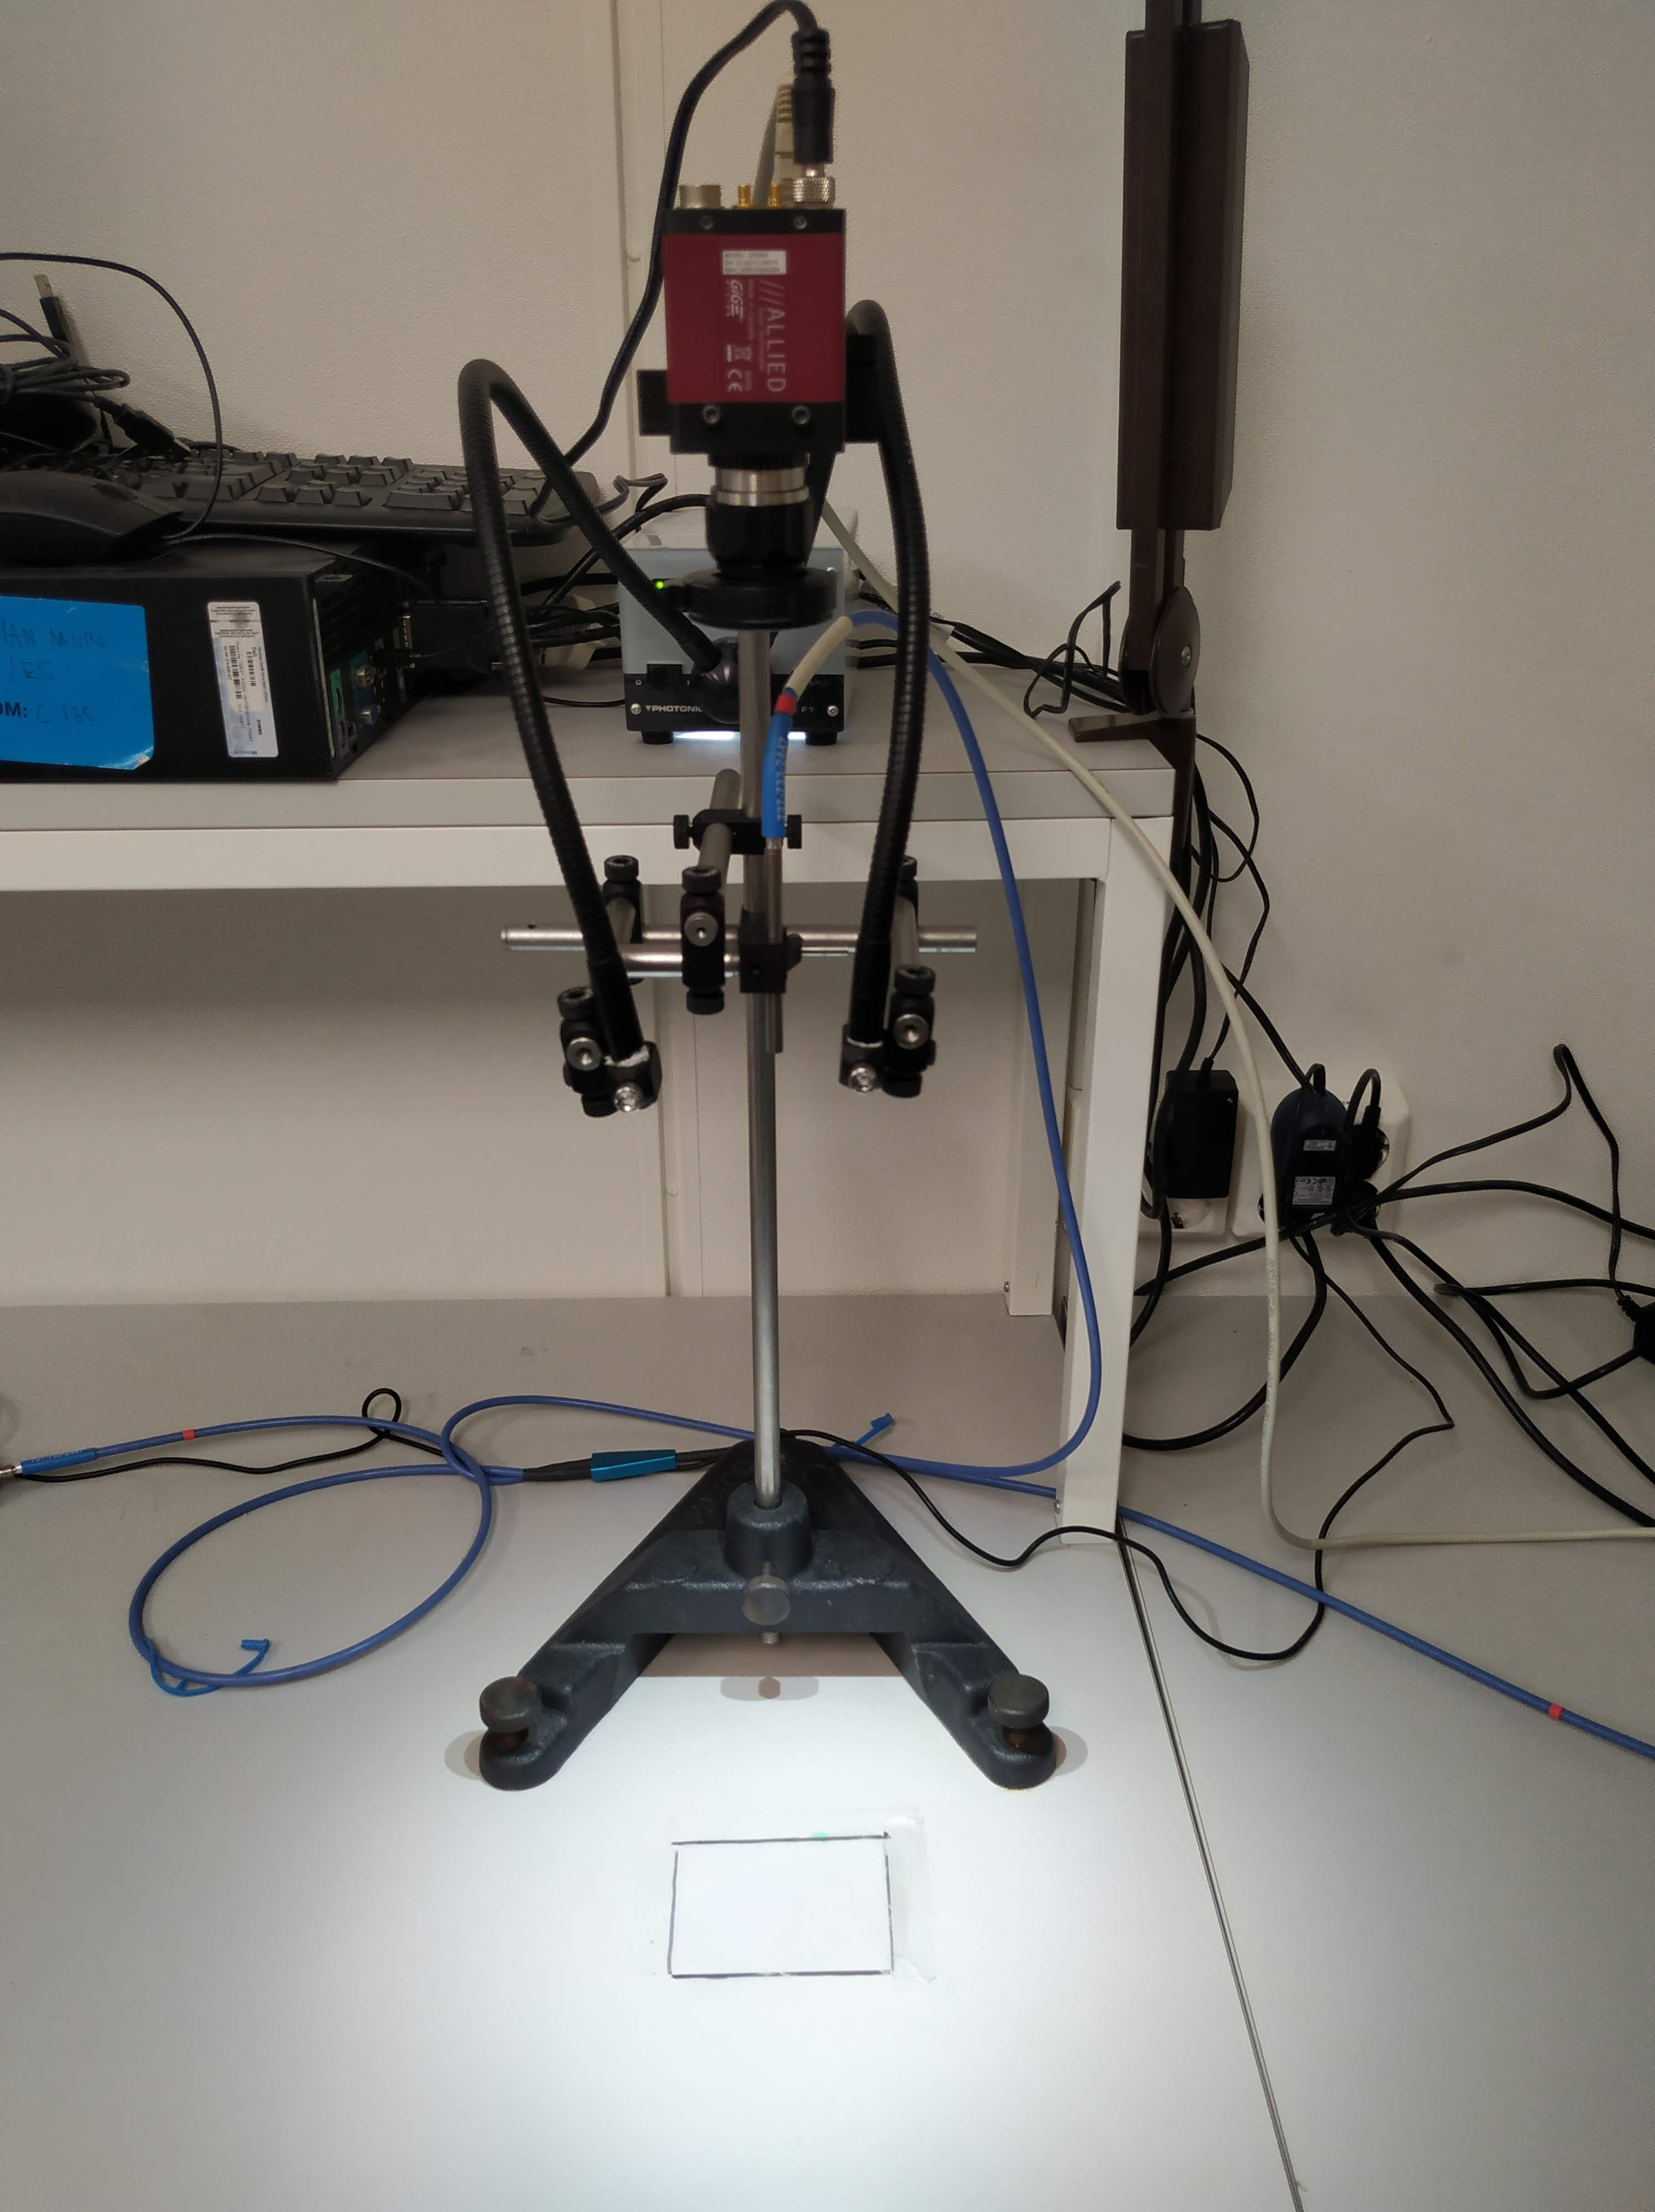
\includegraphics[width=0.95\linewidth]{figures/project_setup_lit.png}
        \caption{Lit room.}
        \label{fig:picture_of_setup_lit}
    \end{subfigure}%
    \begin{subfigure}{0.3333\textwidth}
        \centering
        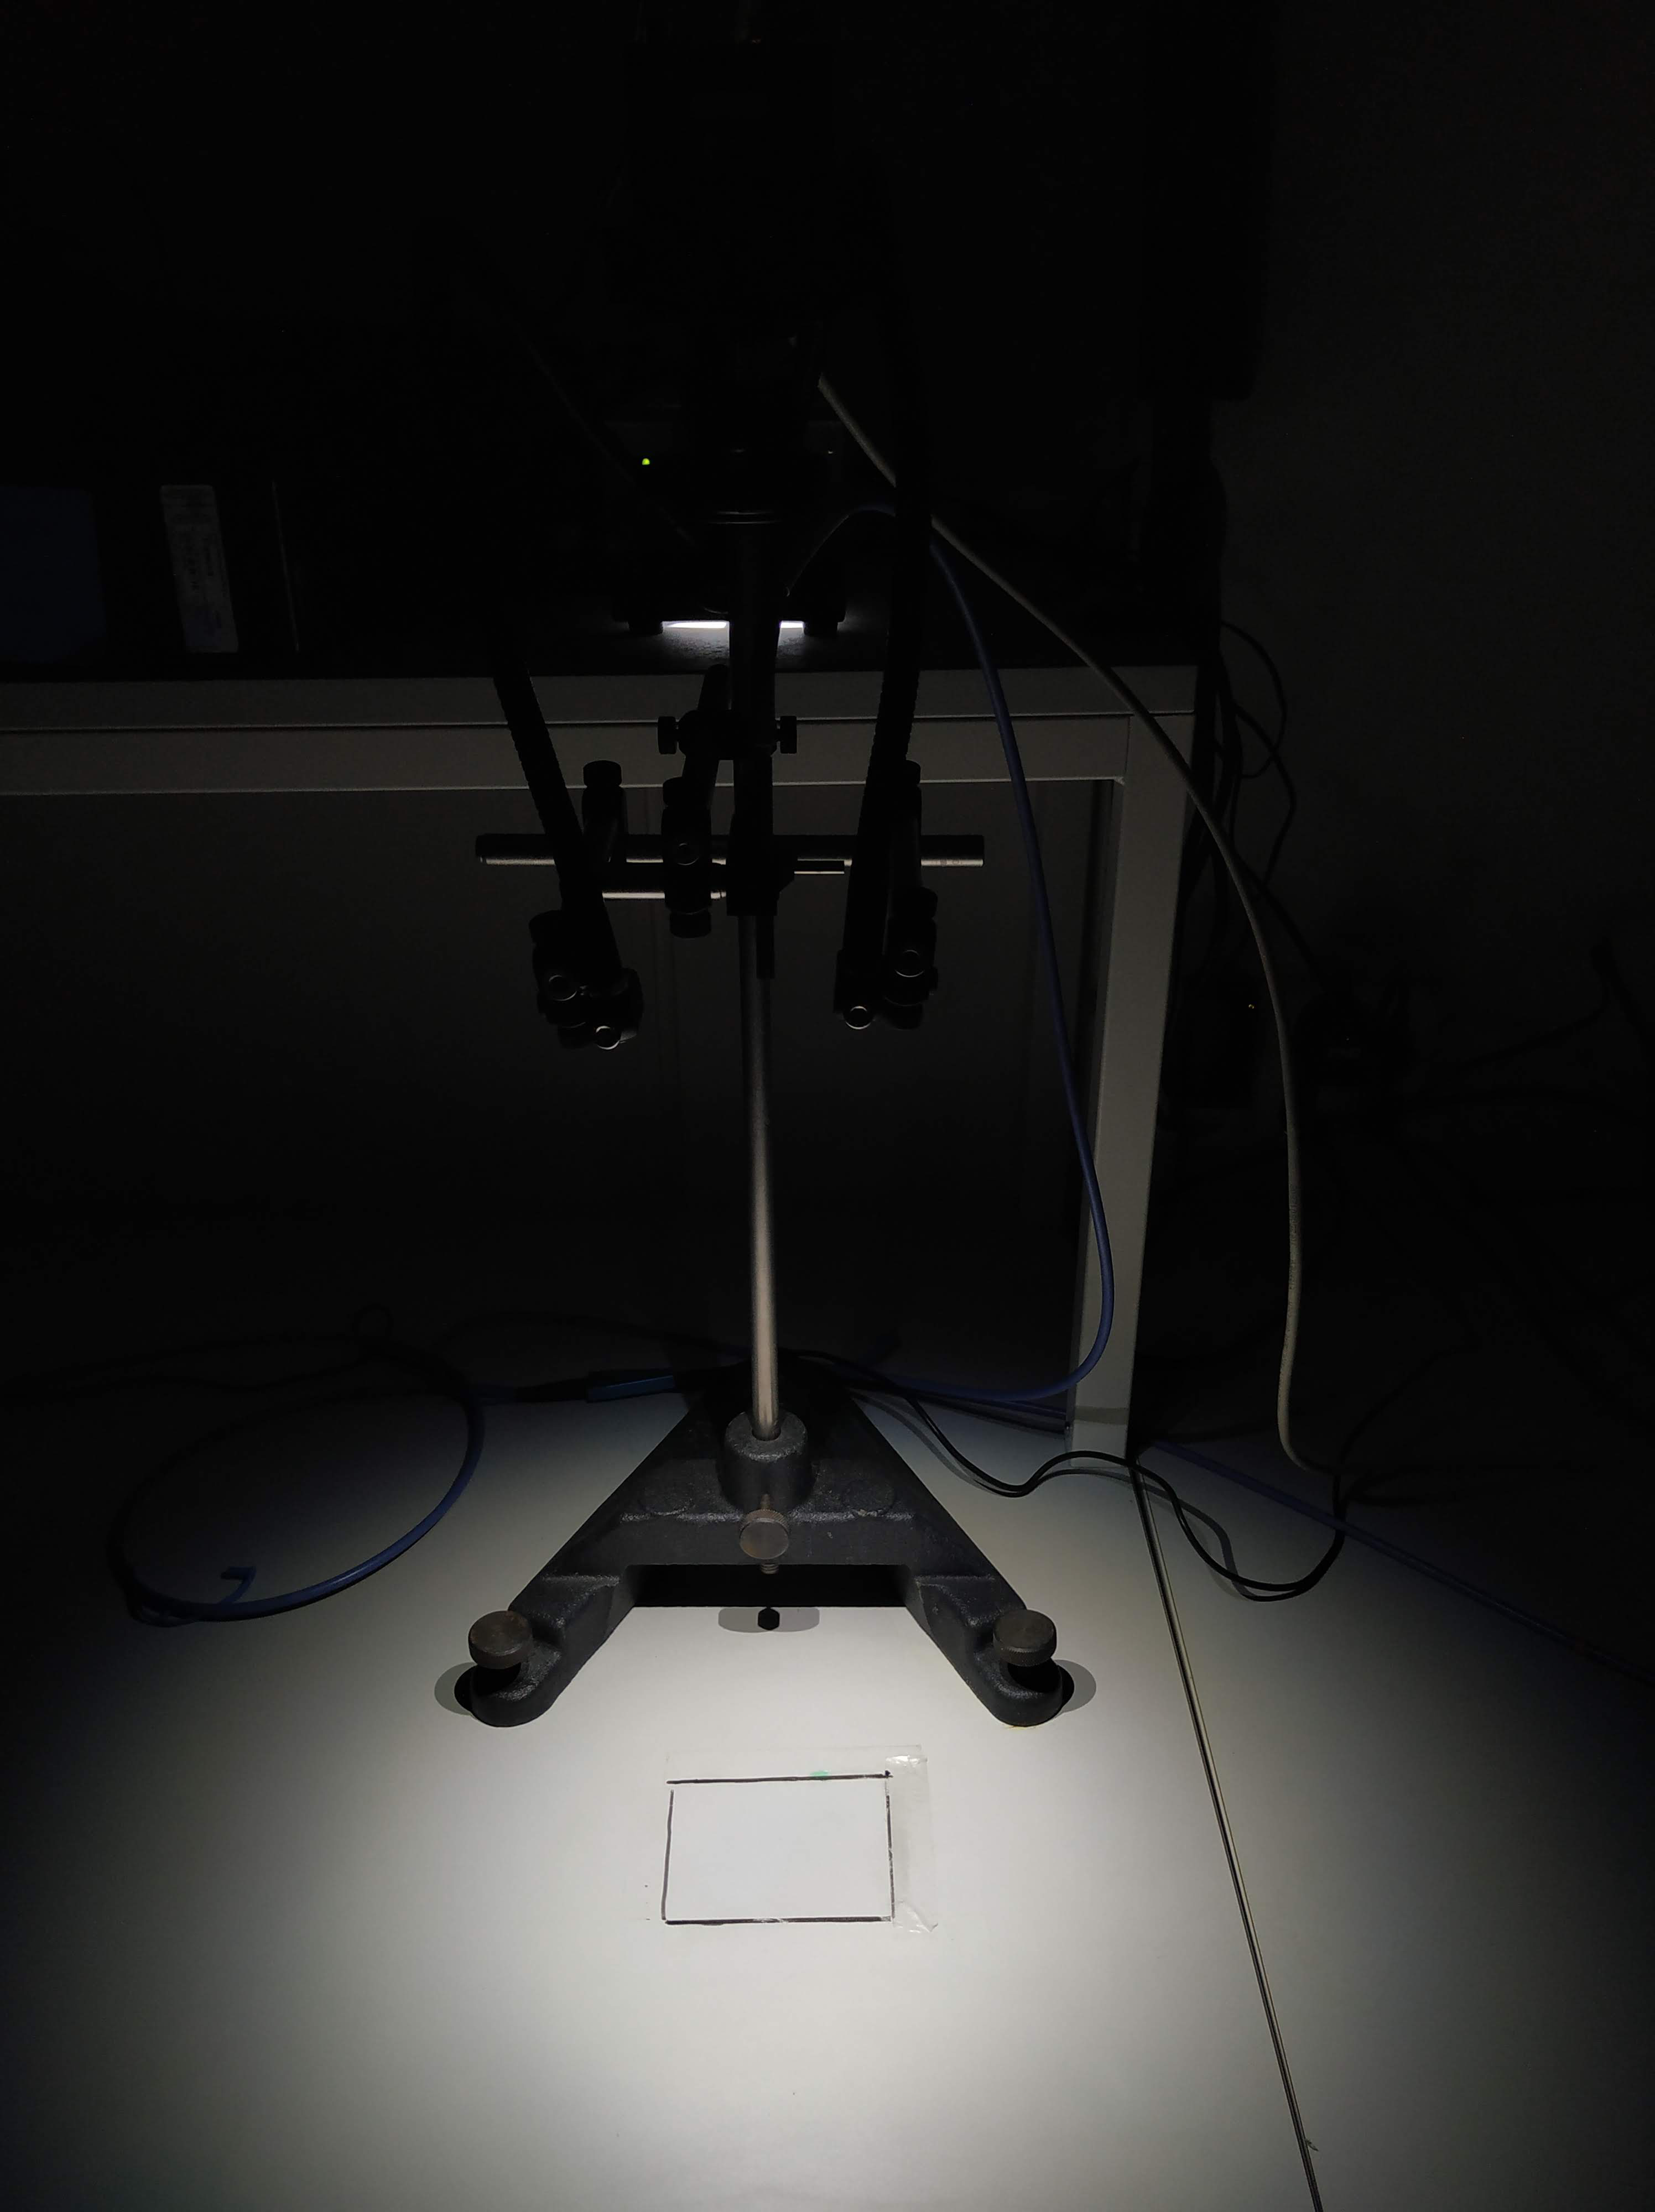
\includegraphics[width=0.95\linewidth]{figures/project_setup_unlit.png}
        \caption{No ambient light.}
        \label{fig:picture_of_setup_unlit}
    \end{subfigure}%
    \begin{subfigure}{0.3333\textwidth}
        \centering
        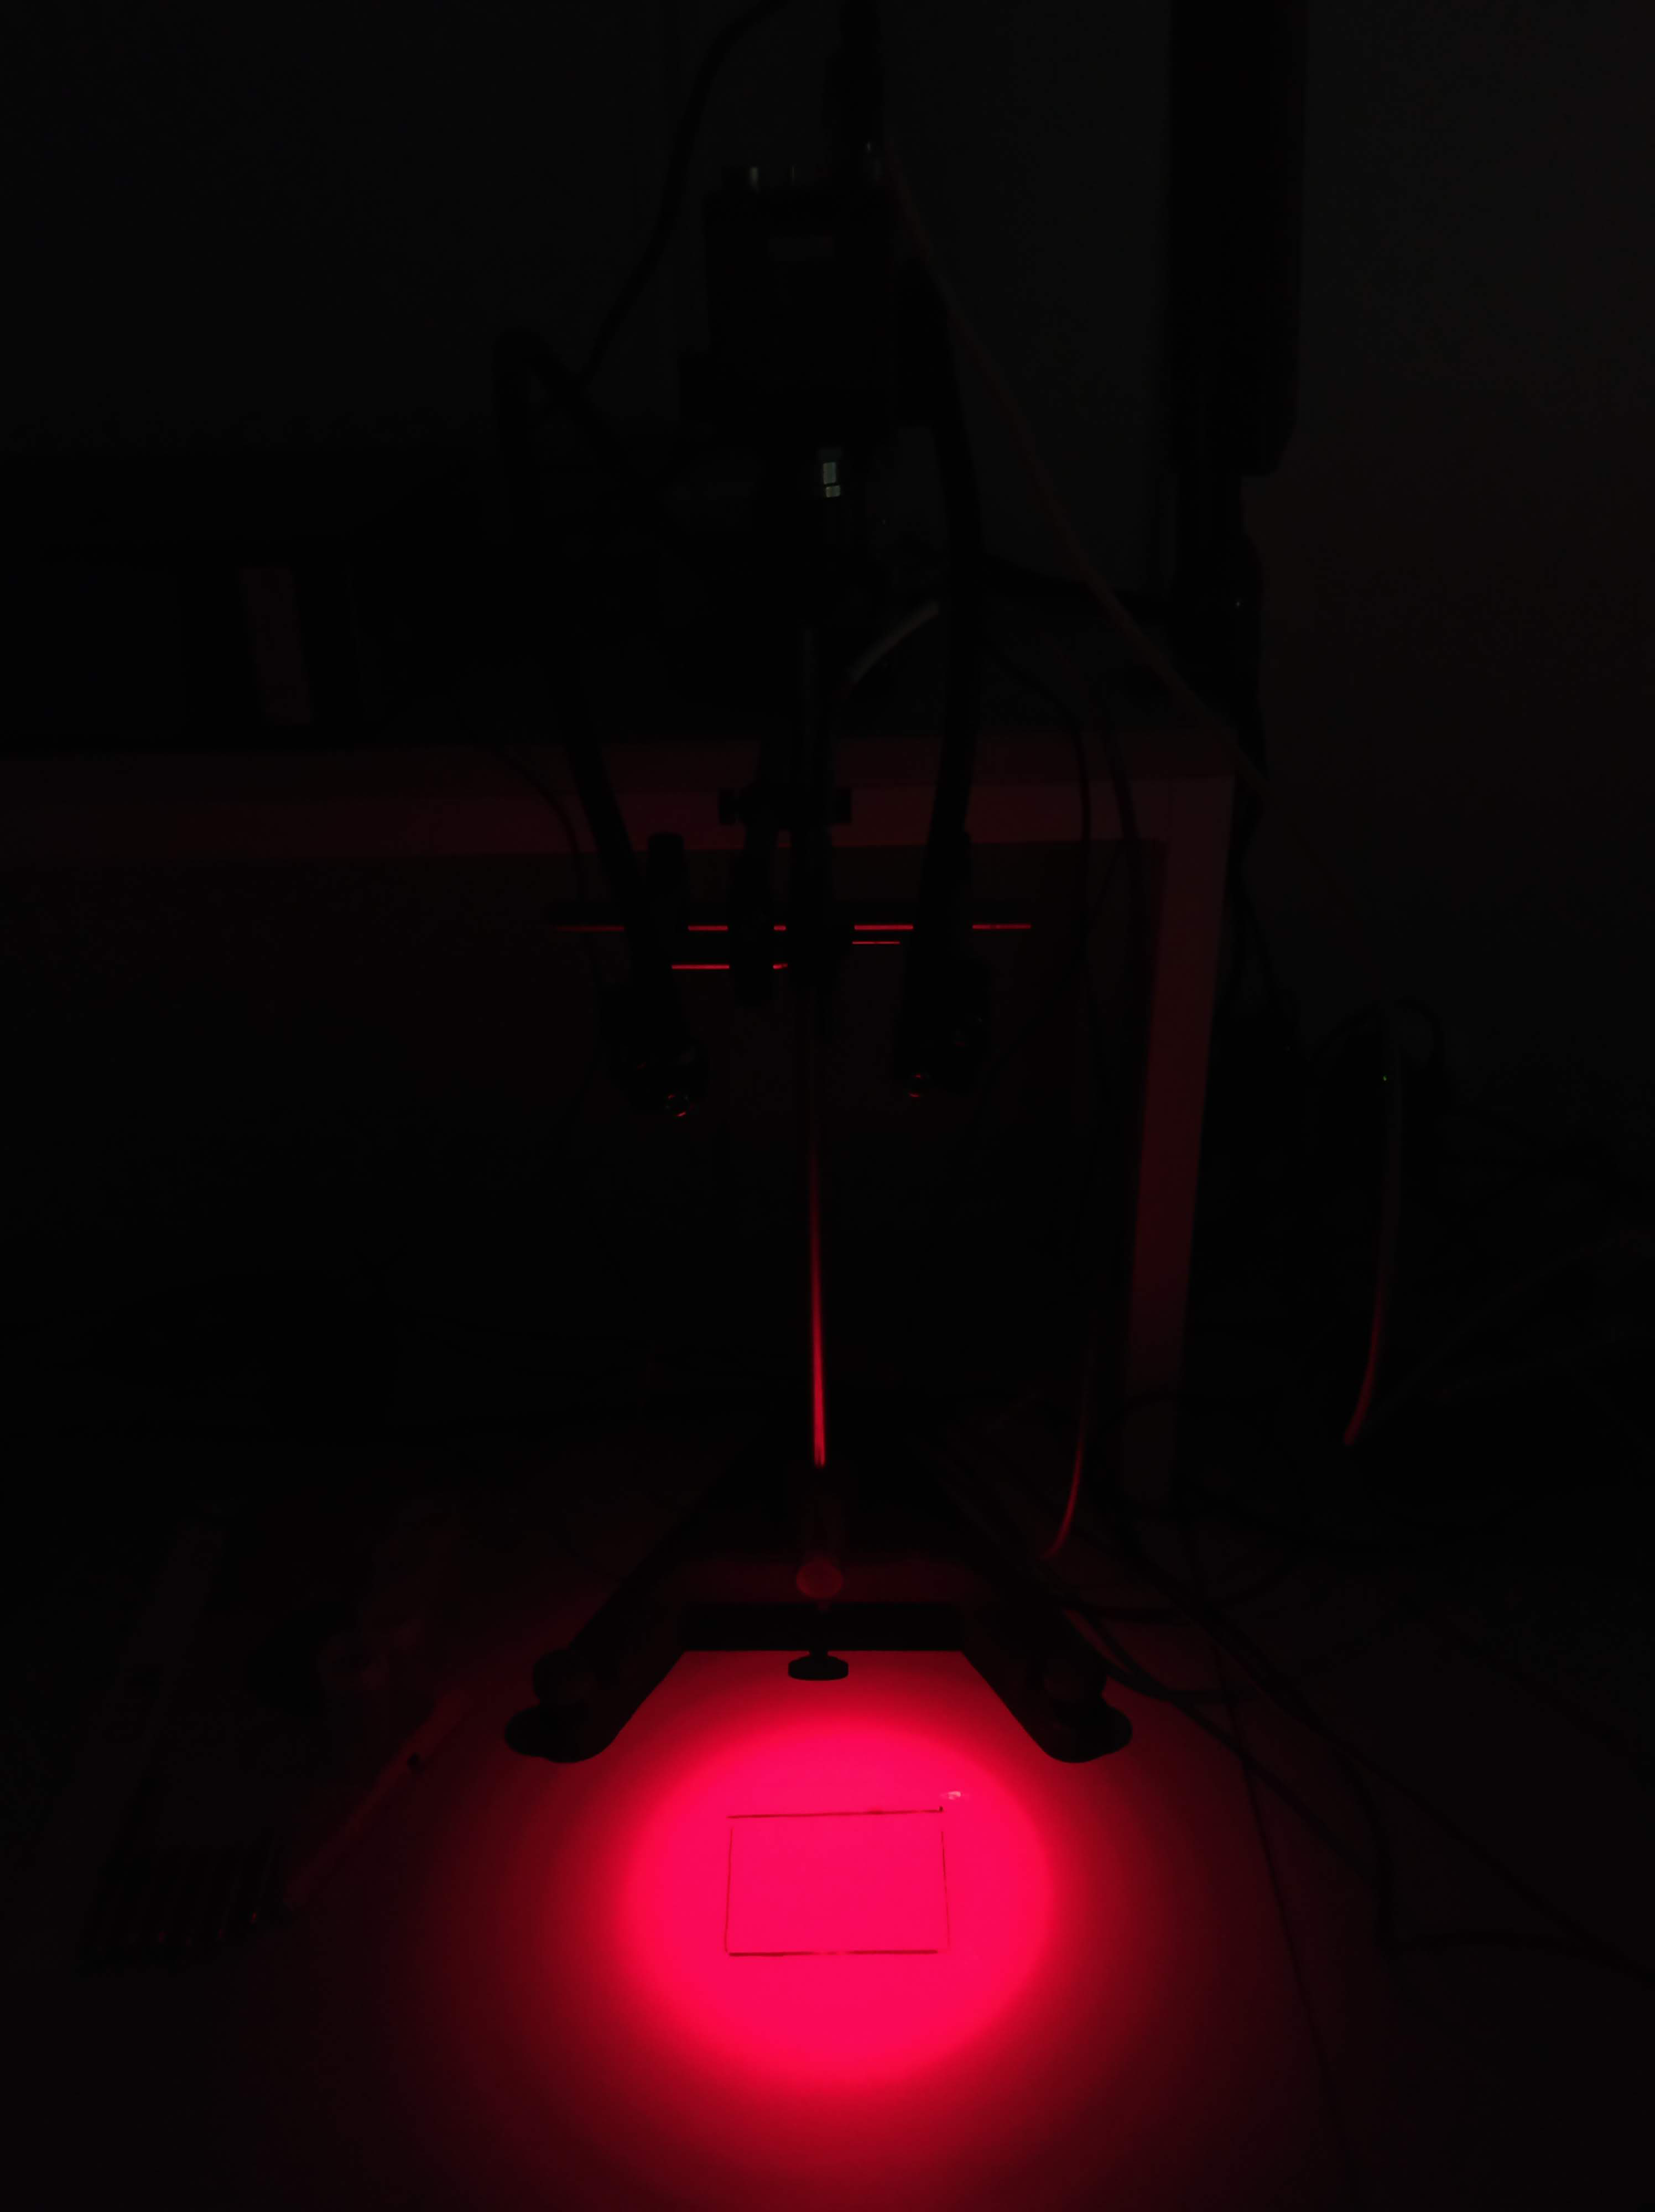
\includegraphics[width=0.95\linewidth]{figures/project_setup_red.png}
        \caption{Red light sent through the fiber.}
        \label{fig:picture_of_setup_red}
    \end{subfigure}
    \caption{Photo of the setup used to take images and spectrums}
    \label{fig:photo_of_setup}
\end{figure}

\subsubsection{Utilities}
The equipment used in the experiment are listed in table 

%TODO make an equipment table
\begin{table}[]
    \begin{tabular}{lll}
    Equipment name & Serial number & Usage \\
                   &               &       \\
                   &               &       \\
                   &               &       \\
                   &               &      
    \end{tabular}
\end{table}

\subsection{Experiment}
\label{sec:experiment}

The experimental stage is divided into two parts, one where the images and spectrums should be taken under the best possible conditions, this is the \textbf{ideal} part. Part two of the experiment is the \textbf{unideal} part, and is divided into three parts that introduces one pertubation each.

\textbf{Ideal analysis.} The purpose of the experiment is to correlate spectral and spatial average under ideal conditions to see how strongly they correlate. Take 30 images and spectrums and compare them to one reference image. These images and spectrums should then be analysed as shown in \ref{sec:method_correlating_spectrum_to_camera}. Fit one linear regression line to each of three colors, then test the amount of error in this approximation. 

\textbf{Unideal analysis}. The purpose here is to create an unideal situation and find what pertubations affects the results. The results shall be compared with the regression lines created in the ideal situation to see if they still fit. The three pertubations that will be introduced are:

\textbf{Ambient light.} In this setup all the light in the lab should be turned on to increase the amount of noise due to the illumination.

\textbf{Border of imaging area.} Here the objects should be placed so that they are only partly inside the imaging area. This should make parts of them only visible to the spectrometer, thus creating a difference in what they will be seeing. 

\textbf{Outside the imaging area.} The same object should be put inside the cameras viewpoint for every image, but a different object should be put just outside of it. It should still be inside the spectrometers view angle.


Four sets of images and spectrum sha